\chapter{Návrh API pro rozvrhová data ÚTVS ČVUT \label{navrh}}

\section{Poskytnuté databázové pohledy}\label{poskytnutuxe9-databuxe1zovuxe9-pohledy}

V~MySQL databázi Ústavu tělesné výchovy a sportu ČVUT v~Praze jsem dostal k~dispozici sadu SQL pohledů, která zpřístupňují data vhodná pro sestavení rozvrhů. Nad těmito pohledy budu navrhovat RESTful službu. V~této části nejprve čtenáře seznámím se strukturou dat. Informace čerpám z~wiki FIT ČVUT v~Praze provozované Oddělením pro rozvoj \autocite{rozvojwiki}.

\subsection{Destinace}\label{destinace}

Destinace pro výcvikové kurzy (vícedenní kurzy mimo areál školy). Struktura je znázorněna \protect\hyperlink{tab:destination}{v~tabulce}.

\begin{longtable}[]{@{}lll@{}}
\caption{Struktura pohledu v\_destination \label{tab:destination}}\tabularnewline
\toprule
Název sloupce & Datový typ & Popis\tabularnewline
\midrule
\endfirsthead
\toprule
Název sloupce & Datový typ & Popis\tabularnewline
\midrule
\endhead
id\_destination & smallint(10) & primární klíč\tabularnewline
name & varchar(50) & název\tabularnewline
url & varchar(250) & URL stránky na utvs.cvut.cz\tabularnewline
\bottomrule
\end{longtable}

\subsection{Haly}\label{haly}

Sportoviště ÚTVS, ve kterých probíhá výuka. Struktura je znázorněna \protect\hyperlink{tab:hall}{v~tabulce}.

\begin{longtable}[]{@{}lll@{}}
\caption{Struktura pohledu v\_hall \label{tab:hall}}\tabularnewline
\toprule
Název sloupce & Datový typ & Popis\tabularnewline
\midrule
\endfirsthead
\toprule
Název sloupce & Datový typ & Popis\tabularnewline
\midrule
\endhead
id\_hall & smallint(6) & primární klíč\tabularnewline
name & varchar(50) & název\tabularnewline
url & varchar(250) & URL stránky na utvs.cvut.cz\tabularnewline
\bottomrule
\end{longtable}

\subsection{Vyučující}\label{vyuux10dujuxedcuxed}

Vyučující jednotlivých kurzů ÚTVS. Struktura je znázorněna \protect\hyperlink{tab:lectors}{v~tabulce}.

\begin{longtable}[]{@{}lll@{}}
\caption{Struktura pohledu v\_lectors \label{tab:lectors}}\tabularnewline
\toprule
Název sloupce & Datový typ & Popis\tabularnewline
\midrule
\endfirsthead
\toprule
Název sloupce & Datový typ & Popis\tabularnewline
\midrule
\endhead
id\_lector & tinyint(10) & primární klíč\tabularnewline
title\_before & varchar(50) & tituly před jménem\tabularnewline
name & varchar(50) & křestní jméno\tabularnewline
surname & varchar(50) & příjmení\tabularnewline
title\_behind & varchar(50) & tituly za jménem\tabularnewline
pers\_number & varchar(20) & osobní číslo (peridno v~KOS)\tabularnewline
url & varchar(250) & URL stránky na utvs.cvut.cz\tabularnewline
\bottomrule
\end{longtable}

\subsection{Sporty}\label{sporty}

Tabulka sportů, které se na ÚTVS praktikují. Struktura je znázorněna \protect\hyperlink{tab:sports}{v~tabulce}.

\begin{longtable}[]{@{}lll@{}}
\caption{Struktura pohledu v\_sports \label{tab:sports}}\tabularnewline
\toprule
Název sloupce & Datový typ & Popis\tabularnewline
\midrule
\endfirsthead
\toprule
Název sloupce & Datový typ & Popis\tabularnewline
\midrule
\endhead
id\_sport & smallint(10) & primární klíč\tabularnewline
short & varchar(50) & kód (tříznaková zkratka)\tabularnewline
sport & varchar(50) & název\tabularnewline
description & text & popis\tabularnewline
\bottomrule
\end{longtable}

\subsection{Zápisy studentů}\label{zuxe1pisy-studentux16f}

V~této tabulce, nepřesně nazvané jako studenti, se eviduje zápis studenta na konkrétní předmět v~daném semestru. V~jednom semestru zde student může mít i více záznamů. Záznamy se po několika letech promazávají. Struktura je znázorněna \protect\hyperlink{tab:students}{v~tabulce}.

Semestr je ve formátu \verb!YYYY/ZZ_S!, kde \verb!YYYY/ZZ! značí akademický rok (např. \verb!2012/13!) a \verb!S! období semestru (1 -- zimní; 2 -- letní).

\begin{longtable}[]{@{}lll@{}}
\caption{Struktura pohledu v\_students \label{tab:students}}\tabularnewline
\toprule
Název sloupce & Datový typ & Popis\tabularnewline
\midrule
\endfirsthead
\toprule
Název sloupce & Datový typ & Popis\tabularnewline
\midrule
\endhead
id\_student & int(11) & primární klíč\tabularnewline
personal\_number & int(11) & osobní číslo (peridno v~KOS)\tabularnewline
kos\_kod & varchar(20) & kód zapsaného předmětu TV v~KOS\tabularnewline
utvs & int(11) & ID zapsaného předmětu ÚTVS\tabularnewline
\begin{minipage}[t]{0.32\columnwidth}\raggedright\strut
\strut
\end{minipage} & \begin{minipage}[t]{0.32\columnwidth}\raggedright\strut
\strut
\end{minipage} & \begin{minipage}[t]{0.32\columnwidth}\raggedright\strut
(v\_subjects.id\_subjects)\strut
\end{minipage}\tabularnewline
semester & varchar(10) & semestr zápisu\tabularnewline
registration\_date & timestamp & datum a čas zápisu\tabularnewline
tour & int(0) & příznak udávající, zda je zapsaný\tabularnewline
\begin{minipage}[t]{0.32\columnwidth}\raggedright\strut
\strut
\end{minipage} & \begin{minipage}[t]{0.32\columnwidth}\raggedright\strut
\strut
\end{minipage} & \begin{minipage}[t]{0.32\columnwidth}\raggedright\strut
předmět kurz\strut
\end{minipage}\tabularnewline
kos\_code & int(0) & příznak udávající, zda kos\_kod\tabularnewline
\begin{minipage}[t]{0.32\columnwidth}\raggedright\strut
\strut
\end{minipage} & \begin{minipage}[t]{0.32\columnwidth}\raggedright\strut
\strut
\end{minipage} & \begin{minipage}[t]{0.32\columnwidth}\raggedright\strut
obsahuje skutečný kód z~KOS\strut
\end{minipage}\tabularnewline
\bottomrule
\end{longtable}

\subsection{Předměty ÚTVS}\label{pux159edmux11bty-uxfatvs}

Předmětem je zde myšlena konkrétní instance vyučovaného sportu, v~daný den a hodinu. Pokud bychom chtěli najít paralelu se systémem KOS, tak tato entita představuje sloučeninu instance předmětu, její paralelky a rozvrhového lístku. Struktura je znázorněna \protect\hyperlink{tab:subjects}{v~tabulce}.

Všimněte si, že některé číselné údaje jsou uloženy textově.

\begin{longtable}[]{@{}lll@{}}
\caption{Struktura pohledu v\_subjects \label{tab:subjects}}\tabularnewline
\toprule
Název sloupce & Datový typ & Popis\tabularnewline
\midrule
\endfirsthead
\toprule
Název sloupce & Datový typ & Popis\tabularnewline
\midrule
\endhead
id\_subjects & smallint(10) & primární klíč\tabularnewline
sport & varchar(10) & ID sportu (v\_sports.id\_sport)\tabularnewline
shortcut & varchar(50) & kód ÚTVS předmětu (např. TUR01)\tabularnewline
day & varchar(10) & den v~týdnu (1–7)\tabularnewline
begin & varchar(10) & čas začátku výuky (HH:MM)\tabularnewline
end & varchar(10) & čas konce výuky (HH:MM)\tabularnewline
hall & varchar(50) & ID haly (v\_hall.id\_hall)\tabularnewline
lector & varchar(50) & ID vyučujícího (v\_lectors.id\_lector)\tabularnewline
notice & text & poznámka (v~HTML)\tabularnewline
semester & tinyint(4) & parita semestru, ve kterém se vypisuje\tabularnewline
\begin{minipage}[t]{0.32\columnwidth}\raggedright\strut
\strut
\end{minipage} & \begin{minipage}[t]{0.32\columnwidth}\raggedright\strut
\strut
\end{minipage} & \begin{minipage}[t]{0.32\columnwidth}\raggedright\strut
(1 -- zimní, 2 -- letní)\strut
\end{minipage}\tabularnewline
\bottomrule
\end{longtable}

\subsection{Diagram}\label{diagram}

\begin{figure}
\centering
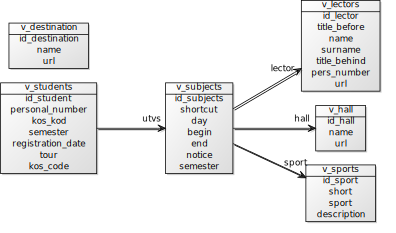
\includegraphics{pdfs/diagram}
\caption{Diagram poskytnutých databázových pohledů \autocite{rozvojwiki}\label{pic:diagram}}
\end{figure}

\protect\hyperlink{pic:diagram}{Na obrázku} můžete vidět diagram vztahů.

\section{API zdroje}\label{api-zdroje}

V~této části navrhnu jednotlivé API zdroje (\emph{resources}) a režim přístupu k~nim. Nebudu se snažit o~striktní návrh, ve kterém bych definoval přesnou podobu odpovědí; to mi umožní nechat přesnou podobu na použitém frameworku. Jednotlivé zdroje budou odpovídat poskytnutým databázovým pohledům.

\subsection{/destinations}\label{destinations}

Poskytne přístup k~datům z~pohledu \verb!v_destination!. Jednotlivě pomocí primárního klíče (\verb!/destinations/{id}!) nebo hromadně. V~odpovědi budou zahrnuta všechna data \protect\hyperlink{tab:destination}{z tabulky}.

\begin{itemize}
\tightlist
\item
  Položka \verb!id_destination! bude přejmenována na \verb!id!.
\end{itemize}

Data budou přístupná pro všechny autentizované klienty.

\subsection{/halls}\label{halls}

Poskytne přístup k~datům z~pohledu \verb!v_hall!. Jednotlivě pomocí primárního klíče (\verb!/halls/{id}!) nebo hromadně. V~odpovědi budou zahrnuta všechna data \protect\hyperlink{tab:hall}{z tabulky}.

\begin{itemize}
\tightlist
\item
  Položka \verb!id_hall! bude přejmenována na \verb!id!.
\end{itemize}

Data budou přístupná pro všechny autentizované klienty.

\subsection{/teachers}\label{teachers}

Poskytne přístup k~datům z~pohledu \verb!v_lectors!. Jednotlivě pomocí primárního klíče (\verb!/teachers/{id}!) nebo hromadně. K~přejmenování dochází kvůli sjednocení s~KOSapi, Siriem a dalšími službami. V~odpovědi budou zahrnuta všechna data \protect\hyperlink{tab:lectors}{z tabulky}.

\begin{itemize}
\tightlist
\item
  Položka \verb!id_lector! bude přejmenována na \verb!id!.
\item
  Položka \verb!pers_number! bude přejmenována na \verb!personal_number!.
\item
  Položka \verb!title_before! bude přejmenována na \verb!degrees_before!.
\item
  Položka \verb!title_behind! bude přejmenována na \verb!degrees_after!.
\item
  Položka \verb!name! bude přejmenována na \verb!first_name!.
\item
  Položka \verb!surname! bude přejmenována na \verb!last_name!.
\end{itemize}

Data budou přístupná pro všechny autentizované klienty.

\subsection{/sports}\label{sports}

Poskytne přístup k~datům z~pohledu \verb!v_sports!. Jednotlivě pomocí primárního klíče (\verb!/sports/{id}!) nebo hromadně. V~odpovědi budou zahrnuta všechna data \protect\hyperlink{tab:sports}{z tabulky}.

\begin{itemize}
\tightlist
\item
  Položka \verb!id_sport! bude přejmenována na \verb!id!.
\item
  Položka \verb!sport! bude přejmenována na \verb!name!.
\item
  Položka \verb!short! bude přejmenována na \verb!shortcut!.
\end{itemize}

Data budou přístupná pro všechny autentizované klienty.

\subsection{/enrollments}\label{enrollments}

Poskytne přístup k~datům z~pohledu \verb!v_students!. Jednotlivě pomocí primárního klíče (\verb!/enrollments/{id}!) nebo hromadně. V~odpovědi budou zahrnuta všechna data \protect\hyperlink{tab:students}{z tabulky} kromě položky \verb!kos_code!.

\begin{itemize}
\tightlist
\item
  Položka \verb!id_student! bude přejmenována na \verb!id!.
\item
  Položka \verb!kos_kod! bude přejmenována na \verb!kos_course_code! a bude nastavena na \emph{null}, pokud je \verb!kos_code! 0.
\item
  Položka \verb!utvs! bude přejmenována na \verb!course! a bude obsahovat odkaz na daný zdroj.
\item
  Položka \verb!tour! bude reprezentována jako boolean.
\end{itemize}

\subsubsection*{Přístupová práva}\label{pux159uxedstupovuxe1-pruxe1va}

\begin{itemize}
\tightlist
\item
  Autentizovaným uživatelům/studentům budou zpřístupněna data o~jejich osobě (osobní číslo musí odpovídat osobnímu číslu přihlášeného uživatele).
\item
  Autentizovaným uživatelům/zaměstnancům budou zpřístupněna všechna data.
\item
  Speciálním autentizovaným klientům budou zpřístupněna všechna data, pro služby jako Sirius a podobné.
\end{itemize}

\subsection{/courses}\label{courses}

Poskytne přístup k~datům z~pohledu \verb!v_subjects!. Jednotlivě pomocí primárního klíče (\verb!/courses/{id}!) nebo hromadně. K~přejmenování dochází kvůli sjednocení s~KOSapi, Siriem a dalšími službami. V~odpovědi budou zahrnuta všechna data \protect\hyperlink{tab:subjects}{z tabulky}.

\begin{itemize}
\tightlist
\item
  Položka \verb!id_subjects! bude přejmenována na \verb!id!.
\item
  Položka \verb!lector! bude přejmenována na \verb!teacher!.
\item
  Položka \verb!begin! bude přejmenována na \verb!starts_at!.
\item
  Položka \verb!end! bude přejmenována na \verb!ends_at!.
\item
  Cizí klíče budou reprezentovány odkazem na daný zdroj.
\end{itemize}

Data budou přístupná pro všechny autentizované klienty.

\subsection{Diagram}\label{diagram-1}

\begin{figure}
\centering
\includegraphics{pdfs/diagram2}
\caption{Diagram API zdrojů\label{pic:diagram2}}
\end{figure}

\protect\hyperlink{pic:diagram2}{Na obrázku} můžete vidět upravený diagram vztahů.
